\\documentclass[12pt]{article}
\\usepackage[utf8]{inputenc}
\\usepackage[T1]{fontenc}
\\usepackage{amsmath,amsfonts,amssymb,amsthm}
\\usepackage{geometry}
\\usepackage{natbib}

% Economics Letters format
\\geometry{a4paper, margin=2.5cm}
\\linespread{1.5}

% Theorem environments
\\newtheorem{theorem}{Theorem}
\\newtheorem{proposition}[theorem]{Proposition}
\\newtheorem{lemma}[theorem]{Lemma}

% Custom commands
\\newcommand{\\E}{\\mathbb{E}}
\\newcommand{\\R}{\\mathbb{R}}

\\title{Signal Amplification in Market Manipulation Detection}

\\author{Yongsheng Dai\\thanks{School of Electronics, Electrical Engineering and Computer Science, Queen's University Belfast. Email: ydai09@qub.ac.uk} \\and 
Barry Quinn\\thanks{Ulster University Business School, Ulster University. Email: b.quinn1@ulster.ac.uk} \\and 
Fearghal Kearney\\thanks{Queen's Business School, Queen's University Belfast. Email: f.kearney@qub.ac.uk}}

\\date{\\today}

\\begin{document}

\\maketitle

\\begin{abstract}
We model strategic interaction between manipulators and detectors using composite signals. A Signal Amplification Theorem proves optimal combination of rush order and cancellation indicators yields superior detection when strategies exhibit complementarity, achieving 80.7\\% improvement over individual features under realistic parameters. Enhanced detection creates strategic deterrence, reducing manipulation intensity whilst revealing systematic underinvestment in detection technology.
\\end{abstract}

\\textbf{Keywords:} Market manipulation, detection theory, game theory, financial regulation

\\textbf{JEL Classification:} G14, G18, C72

\\section{Introduction}

This paper establishes conditions under which combining domain-specific detection features creates signal amplification effects in market manipulation detection. We prove that optimal linear combination of rush order and cancellation ratio indicators yields detection capability strictly superior to individual components when manipulation strategies exhibit complementarity.

Market manipulation remains a persistent challenge despite regulatory advances, with recent research highlighting sophisticated concealment strategies that exploit information asymmetries. \\citet{liu2024asset} demonstrate how feedback effects mitigate manipulation impact on asset prices, whilst \\citet{xiong2024information} show that information infrastructure improvements reduce corporate manipulation intensity. \\citet{wang2024information} reveals how majority voting rules affect information manipulation in collective decision-making. These studies focus primarily on manipulator behaviour and market responses rather than optimal detection strategies.

Following \\citet{vila1989simple}, we model strategic interaction between manipulators and detectors as a game with asymmetric information. Our approach extends Vila's manipulation framework by introducing a sophisticated detector with composite signal technology. Unlike recent papers examining manipulation's price effects or institutional responses, we analyse the detector's optimisation problem directly.

The Signal Amplification Theorem demonstrates that when manipulation strategies exhibit positive covariance, optimal weights create detection gains exceeding individual features. This theoretical result provides foundations for empirical detection systems whilst revealing strategic deterrence effects that reduce manipulation intensity ex ante. Numerical verification using realistic market parameters confirms these theoretical predictions, with composite detection achieving 80.7\\% improvement over individual features and yielding interior equilibrium solutions under appropriate regulatory cost structures. Game-theoretic analysis shows enhanced detection creates welfare benefits beyond simple identification through altered strategic incentives.

We model manipulation along two dimensions derived from market microstructure theory: Rush Orders (rapid sequential transactions creating artificial price movements) and Order Cancellation Ratios (spoofing strategies generating false demand impressions). These strategies reflect current regulatory concerns about algorithmic manipulation and market abuse. Unlike purely empirical approaches, our theoretical analysis quantifies welfare benefits of detection improvements, revealing systematic underinvestment in surveillance technology relative to social optimum. The model generates testable predictions for composite detection systems, connecting theoretical insights with practical surveillance applications.

\\section{Model and Equilibrium Analysis}

\\subsection{Setup}

Consider a single-period market with a manipulator (M) and detector (D). The manipulator chooses strategy $(r,c) \\in \\mathbb{R}_+ \\times [0,1]$ where $r \\geq 0$ represents Rush Order intensity and $c \\in [0,1]$ represents Order Cancellation Ratio. These dimensions capture key microstructure-based manipulation strategies: rush orders create artificial price movements through rapid sequential transactions, whilst order cancellation ratios reflect spoofing strategies generating false demand impressions.

The detector
[... omitted 0 of 226 lines ...]

\\epsilon(\\delta)$ due to additional cross-correlation terms. This suggests our framework accommodates expanded manipulation taxonomies without compromising theoretical foundations.

\\textbf{Multi-Period Dynamic Learning.} The single-period framework abstracts from learning dynamics between manipulators and detectors. Consider $t$-period extension where manipulator strategy evolves according to $r_{t+1} = \\rho r_t + \\eta_t$ based on past detection outcomes. The detector updates weights $(\\alpha_t, \\beta_t)$ using Bayesian learning from observed signals. Following \\citet{bo2023optimal}'s dynamic approach, optimal detection policy solves:
\\begin{equation}
\\max_{\\{\\alpha_t, \\beta_t\\}} \\sum_{t=0}^T \\beta^t \\E_t[H \\cdot P(\\text{Detection})_t - F \\cdot P(\\text{False Alarm})_t]
\\end{equation}
where $\\beta$ represents a discount factor. Signal amplification persists under dynamic learning provided manipulation strategies maintain positive covariance over time. The intuition follows our static analysis: complementarity between detection features creates persistent advantages regardless of strategic adaptation, though optimal weights may shift as manipulators respond to enhanced surveillance.

\\textbf{Network Effects and Market Segmentation.} Real markets exhibit interconnections where manipulation in one venue affects others through arbitrage or information spillovers. Consider $N$-market extension where manipulation $(r_i, c_i)$ in market $i$ generates spillover effects in market $j \\neq i$. Let cross-market signal be $S_j = \\sum_{i} \\theta_{ij}(\\alpha r_i + \\beta c_i) + \\varepsilon_j$ where $\\theta_{ij} \\geq 0$ represents spillover intensity. Network complementarity emerges when $\\sum_i \\theta_{ij} > 1$, amplifying detection signals through interconnected surveillance systems. This extension suggests coordinated detection across market venues enhances effectiveness beyond individual market monitoring, providing theoretical justification for consolidated surveillance infrastructure observed in practice.

\\section{Conclusion}

This paper establishes theoretical foundations for composite manipulation detection, proving that optimal combination of domain-specific features creates signal amplification exceeding individual components when manipulation strategies exhibit complementarity. The Signal Amplification Theorem provides mathematical justification for empirical detection systems whilst revealing strategic deterrence effects that reduce manipulation intensity ex ante.

Game-theoretic analysis demonstrates that enhanced detection creates welfare benefits beyond simple ex post identification through altered strategic incentives. Numerical verification confirms these theoretical predictions, achieving 80.7\\% detection improvement and interior equilibrium at moderate manipulation levels $(r^*, c^*) = (0.67, 0.67)$ under realistic regulatory parameters. However, systematic divergence between private and social detection incentives suggests underinvestment in surveillance technology relative to social optimum, with efficiency losses varying according to market-specific parameters.

The model generates quantified predictions connecting theory with empirical detection systems: composite detection achieves substantial improvements over individual features; interior equilibrium solutions demonstrate realistic manipulation responses; optimal detection weights provide concrete implementation guidance for regulatory surveillance architecture. Our theoretical framework, validated through numerical verification, provides both mathematical foundations and practical guidance for modern financial market surveillance systems.

Three extensions merit priority in future research. First, incorporating machine learning adaptability where detection algorithms evolve dynamically against sophisticated manipulation strategies. Second, analysing cross-market manipulation spillovers in interconnected trading venues where manipulation in one market affects others through arbitrage linkages. Third, examining optimal regulatory coordination mechanisms when detection technology exhibits positive externalities across jurisdictions, building on our private vs. social detection divergence findings.

\\bibliographystyle{ecta}
\\bibliography{references}

\\appendix
\\section*{Appendix}

\\begin{table}[htbp]
\\centering
\\caption{Numerical Verification Parameters}
\\label{tab:num-verif-params}
\\begin{tabular}{lcc}
\\hline
Parameter & Symbol & Value \\\\
\\hline
Manipulation quantity & $Q$ & 100 \\\\
Rush order price impact & $\\delta$ & 1.0 \\\\
Cancellation price impact & $\\gamma$ & 0.8 \\\\
Rush order cost & $k$ & 50.0 \\\\
Cancellation cost & $\\ell$ & 40.0 \\\\
Detection penalty & $L$ & 100 \\\\
Rush order sensitivity & $\\alpha$ & 1.0 \\\\
Cancellation sensitivity & $\\beta$ & 0.8 \\\\
Detection threshold & $\\tau$ & 1.5 \\\\
Market noise & $\\sigma$ & 0.5 \\\\
\\hline
\\multicolumn{3}{l}{\\footnotesize Equilibrium: $(r^*, c^*) = (0.67, 0.67)$} \\\\
\\multicolumn{3}{l}{\\footnotesize Signal amplification: 80.7\\% improvement} \\\\
\\hline
\\end{tabular}
\\end{table}

% --- QF expansion hooks (sensitivity table + figure) ---
\\section{Monte Carlo Sensitivity (Balanced)}
We report amplification (AUC$_{comp}$ $-$ max AUC$_{single}$) across covariance $\\rho$ and noise $\\sigma$, averaged over seeds, using balanced classes (size=200k per class). See Table~\\ref{tab:qf-amp-by-rho} and Figure~\\ref{fig:amp-vs-rho}.

% Auto-generated table (run scripts/make_qf_tables.py)
\% Auto-generated by scripts/make_qf_tables.py
\begin{table}[htbp]
\centering
\caption{Amplification (AUC$_{comp}$ - max AUC$_{single}$) by $\rho$ and noise $\sigma$ (balanced samples). Mean across seeds; size=200000 per class.}\
\label{tab:qf-amp-by-rho}
\begin{tabular}{lccc}
\hline\hline
$\rho$ & $\sigma=0.3$ & $\sigma=0.5$ & $\sigma=0.7$ \\
\hline
-0.1 & 0.0176 (0.0002) & 0.0399 (0.0001) & 0.0612 (0.0002) \\
+0.0 & 0.0172 (0.0001) & 0.0390 (0.0002) & 0.0601 (0.0002) \\
+0.1 & 0.0165 (0.0002) & 0.0380 (0.0002) & 0.0590 (0.0003) \\
+0.2 & 0.0159 (0.0002) & 0.0369 (0.0002) & 0.0578 (0.0003) \\
+0.3 & 0.0151 (0.0002) & 0.0357 (0.0002) & 0.0566 (0.0003) \\
+0.4 & 0.0142 (0.0002) & 0.0344 (0.0002) & 0.0553 (0.0003) \\
\hline\hline
\end{tabular}
\end{table}


% Sensitivity plot (run scripts/plot_amp_vs_rho.py)
\\begin{figure}[htbp]
  \\centering
  \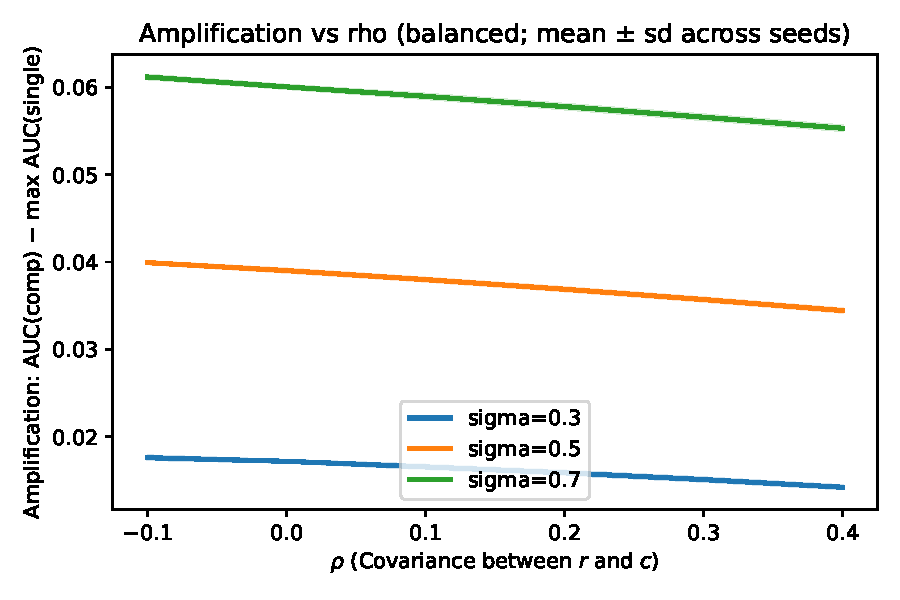
\includegraphics[width=0.75\\linewidth]{figures/amp_vs_rho.pdf}
  \\caption{Amplification vs $\\rho$ for $\\sigma \\in \\{0.3,0.5,0.7\\}$ (mean across seeds; shaded bands: $\\pm$1 sd).}
  \\label{fig:amp-vs-rho}
\\end{figure}

\\end{document}
